\begin{center}
    {\huge  Análise da interação Hospedeiro-parasitóide}
    
    \medskip
    
    {\large Daniel Ambrosim Falqueto e Darlan Augusto Farias Araújo}
    
    \medskip
    
    FGV - Fundação Getúlio Vargas, setembro de 2022
\end{center}

\section{Resumo}

O modelo matemático hospedeiro-parasitóide é um modelo que foi desenvolvido com o objetivo de entender as interações de uma ou mais espécies de hospedeiros para um respectivo parasita que em sua maioria são Insetos. O objetivo de modelar tais interações se deve ao fato de que o controle biológico de pragas, que em sua maioria são insetos, é muito necessário já que se não houver o controle desse tipo de praga, um enorme prejuízo pode ser causado, sejam eles para própria natureza ou para o ser humano. A modelagem dessa interação permite a tomada de uma contramedida, em sua maioria um controle biológico clássico, onde o dano que esses seres causam é controlado com a adição de um inimigo natural desse parasita, que reduziria a população desse mesmo ser. Esse método é um dos mais eficientes já que não é um meio de redução químico ou não natural.

\section{Por que combinar modelagem ecológica com controle da população de pragas?}

Geralmente, os padrões de ciclos, picos ou crashes ecológicos das tendências populacionais estão fortemente associados a doenças endógenas e/
ou forças exógenas. Por isso a relção ou correlação dessas forças com a abundância populacional tem sido muito estudadas nas últimas dácadas. Além disso, o bioma terrestre passou por intensas e rápidas mudanças, principalmente desde o século passado por causa da ação humana, provavelmente resultando em novos padrões ecológicos como resultado da pressão exercida por essas mudanças nos organismos.

A expressão “mundo em mudança” está presente ou implícita em muitos jornais, revistas, jornais, ou mesmo títulos de reuniões científicas. Particularmente, na entomologia há uma crescente preocupação com o mundo em mudança associado à surtos de pragas, ruídos ambientais, invasões biológicas e o estabelecimento de espécies exóticas em novas áreas. Essa preocupação decorre da saúde humana e animal, o papel dos insetos na agricultura, juntamente com os integrantes essenciais da biodiversidade. Os efeitos das mudanças no mundo são refletidas nas dinâmicas populacionais e investigar transformações rápidas não é um trabalho trivial pelo menos para entende-los em sua totalidade.

Um modelo matemático é essencialmente uma caricatura de um sistema e pode funcionar como um importante protótipo a ser investigado, principalmente por causa de sua estrutura simples. O primeiro passo para modelar os sistemas é entender parcialmente modelos complexos, porque uma característica importante dos modelos é sua flexibilidade. Vamos tentar mostrar quais são os principais pontos listados atualmente pelos ecologistas e entomologistas, que podem impedir a compreensão do comportamento da população de insetos e, consequentemente, a implementação do Manejo Integrado de Pragas (MIP).

\section{Suprimento de comida e insetos}

Um dos maiores impecílios da humanidade em relação a produção de alimentos, tarefa que por si só é desafiadora, são as pragas. Durante vários anos a humanidade encontrou modos para lidar com essa categoria de criatura, apesar de que a maioria dos métodos resultava não só no extermínio desses seres, mas também em uma transformação drásticamente nociva no ambiente, fauna, flora e por consequência no próprio ser humano. Exemplos dessas soluções são os agrotóxicos, que apesar de fazer seu trabalho de exestermínio com sucesso, acabam por gerar um dano residual no ambiente em que são aplicados, afentando a vegetação, animais, rios, lagos e etc. Causando um ano na própria natureza que pode ser incalculável.

O deselvolvimento humano e a oferta alimentar são conceitos que devem estar de mãos dadas, porém não é isso que anda acontecendo recentemente no mundo, criando uma dependência no aumento de recursos alimentares, que por sua vez resulta em uma necessidade na redução criada pelas pragas. Além da necessidade no aumento dos niveis atuais em relação a produção de alimentos, causado pela crescente desnutrição humana no mundo inteiro.

O avanço tecnológico tem sido de grande contribuição para o aumento da eficiência da agricultura, principalmente quando se trata de alimentos trangênicos, ao usar da ciência para alterar o DNA das plantas, melhorando sua variabilidade genética, resultando em maior resistência a doenças e maior tempo de vida. Porém, mesmo isso não é necessário para controlar a enorme demanda da humanidade por alimentos, algo que gerará prejuízos futuramente. Esses fatos são colocados a mesa sem contar o prejuízo causado por pragas, o que geraria um futuro realmente péssimo na perspectiva humana.


\section{Pesticidas e MIP}

Um dos desafios desse século é tentar controlar o avanço de insetos e pragas. Uma das tentativas é o uso de pesticidas que, quando utilizados em excesso, contaminam alimentos, o meio ambiente e acabam eliminando também outros insetos que são inimigos naturais das pragas e não prejudicam a produção dos alimentos. Porém utilizar um inimigo natural especializado tem a desvantagem fundamental de que dificilmente pode erradicar a praga alvo, a menos que a primeira seja altamente vulnerável a um efeito específico. 

Por isso novas técnicas tem sido desenvolvidas, como variedades resistentes, rotação de culturas e lavouras, fertilização, saneamento, culturas com armadilhas, poda, etc. Além disso aumento e soltagem de predadores naturais, parasitóides e/ou patógenos também começaram a ser utilizados. Em particular, técnicas genéticas, como liberação de insetos estéreis e organismos modificados estão em intenso desenvolvimento para aplicação imediata. Embora a importância do novo cenário seja reconhecida a falta de dados para o modelo dificulta a modelagem precisa da utilização dos pesticidas modernos e os métodos de controle acima mencionados sobre pragas de insetos, bem como na saúde humana e no ambiente. 

Para compensar parcialmente os efeitos negativos pré-mencionados do uso de um inimigo natural especializado, uma abordagem promissora é implementar um conjunto multi-inimigo em vez de um único agente de biocontrole. A previsão é encorajadora para o uso do paradigma de assemblage multi-inimigo no manejo de pragas. No entanto, o
questão prática central, que permanece obscura, é sobre a alteração do tamanho da população do alvo
pragas após o biocontrole, ou seja, se o uso de vários agentes reduzirá bastante o impacto negativo
da praga no meio ambiente. De fato, os estudos teóricos existentes sobre as coinfecções estão principalmente focados em
a evolução da virulência, prevalência da doença ou a derivação do número básico de reprodução

\section{Aquecimento global e Insetos}
Devido ao crescente aumento do aquecimento global associado aos gases do efeito estufa, tanto fauna quanto flora se vem em constante mudança devido ao fenômeno, influenciando a demografia, geração e interação com plantas das ditas pragas, afetando então diretamente as dinâmicas hospedeiro-parasitóide, de produção de alimentos e de proliferação de doenças. Os anos se passam e os danos causadas pelas pragas aumenta, em conjunto o aquecimento global causa enormes perdas florestais, que não só podem ser concequências do fenômeno, mas também ter influência humana, isso tudo resulta no aumento da geração das pragas.
Um exemplo é o mosquito Aedes aegypti, onde foi analisado por Kearney (2009), que em diferentes regiões termicas da Australia o inseto se reproduz de maneira mais intensa. Isso pode significar que doenças transmitidas por insetos podem começar a surgir em novas áreas em decorrência das mudanças de temperatura. Isso fica mais evidente ao aumento de casos de doenças importadas como a própria dengue.


\section{Cenários, Teoria Ecológica e MIP}

A complexidade da natureza é um cenário atraente para a aplicação de raciocínios complexos e ferramentas analíticas sofisticadas. O desafio que surge é como conectar a ciência teórica com os experimentos para medir e melhorar a produção sem causar danos a natureza. A mudança ao longo do tempo das populações de insetos pode exibir padrões ecológicos que podem descrever tendências importantes que pode indicar suscetibilidade a falhas ou surtos. 
Outra questão importante é entender como e quando vai ocorrer uma explosão de insetos, algo que infelizmente é difícil de se prever. Programas de manejo populacional de pragas e insetos vêm sendo implementados há décadas na tentativa de controlar pragas. No entanto, na prática, raramente os programas incorporam todos os componentes que são necessários para avaliar periodicamente o estado das pragas. O manejo de espécies de pragas também implica a análise de padrões ecológicos investigando a frequência de distribuição de insetos para avaliar o padrão de dispersão espacial e desenvolver planos de decisão. Os planos para amostragem de populações de insetos levam em consideração pelo menos três componentes: densidade populacional das pragas, limiar econômico e a previsão dos fenômenos.

\section{Artigos com modelagem relacionada}

O artigo "Ecological Modeling and Pest Population Management" (1), explica como Tang & Cheke (2008) estenderam o clássico modelo hospedeiro-parasitóide, incluindo o programa de controle de Manejo Integrado de Pragas (MIP) para considerar o limiar econômico como um componente da formulação. Os resultados encontrados neste estudo sugerem que é possível manter o nível de host abaixo do limiar econômico (LE), evitando o nível de prejuízo econômico (NPE). Além disso, eles mostraram que uma alta densidade inicial de parasitóides, bem como alta sobrevivência intergeracional parasitóide pode influenciar o padrão ecológico da série temporal. Nos programas de MIP, geralmente tanto a pulverização de pesticidas quanto a liberação de parasitóides ocorre quando a densidade populacional do hospedeiro atinge o limiar econômico para manter a densidade do hospedeiro abaixo do NPE. 

Fazendo simulações, para cada geração, a dinâmica consiste em duas fases: fase de dispersão e fase de reprodução-parasitismo. A taxa de mortalidade instantânea em resposta ao pesticida pode ser estimado, e somando-o ao caso pode melhorar as estratégias de MIP, determinando tanto o período ótimo de aplicações e a porcentagem de pragas que
precisam ser eliminados com pesticidas. Os resultados apresentados sugerem que para o sucesso das estratégias de MIP, a estrutura espacial dos sistemas deve ser levado em consideração nos programas de controle de pragas, pois migração entre as populações locais pode anular o efeito produzido pelo LE. Não existe um estudo sistemático explorando a conexão entre as estratégias de IPM e a estrutura espacial. 

\medskip

Outro artigo "Ecological Modeling and Pest Population Management" (2), aprensenta que o controle biológico tem como um dos seus pricipais objetivos o controle de pragas por meio de predadores/inimigos naturais, por ser uma maneira de lidar com as pragas efetiva e que não altera drasticamente o meio ambiente. Sendo sempre melhor o uso de varios desses inimigos ao em vez de usar apenas uma única espécie, porém atualmente a pouca modelagem dos resultados da utilização de vários inimigos como meio de controle biológico para pragas, apesar da existência de muitos estudos téoricos em diversas áreas da biologia, pricipalmente em ecologia e epidemiologia, sobre o assunto. O Trabalho, tem como princial objetivo provar que a eficiencia do controle de pragas por meio do controle biológico e o número de inimigos naturais utilizados nesse controle é proporcional.

Nesse trabalho, foi implementado uma modelagem baseada em teoria dos jogos de dinâmica adaptativa, descobrindo que o aumento do número da variedade de espécies inimigas de uma dada praga, faz com que a mesma tenha sua mortalidade reduzida. Apesar de que em alguns casos a mudança pode ser mínima ou nula, dependendo se a adição de espécies ser excessiva. Também mostraram a possibilidade de extinção das espécies no avanço da experiência, além de mostrar coexistencia de várias espécies perto de serem extintas. 

\medskip

A troca de hospedeiros no modelo hospedeiro-parasitóide é o principal assunto tratado no artigo "Multiple host use and the dynamics of host switching in host–parasite systems" (3). Ele apresenta  modelos populacionais simples que contém duas espécies de hospedeiros dintintos, onde é observado a adequação do parasita nesses dois diferentes hospedeiros. O foco dessa troca de hospedeiros foi analisada quando a frequência de hospedeiros sobre mudanças, concluindo que tal mudança ocorre de maneira incrivelmente rápida, quedas no número de parasitas podem ocorre graças a essa mudança de hospedeiros e que é de suma importância considerar essas possíveis mudanças de hospedeiros em qualquer dinâmica baseada na interação hospedeiro-parasitóide.

\section{Metodologia}

A teoria do controle biológico de insetos tem uma história associada
com ecologia teórica, pricipalmente se tratando de interações entre um hospedeiro e um parasitóide. O quadro para modelos hospedeiro-parasitóides pode ser descrito a partir de diversos modelos. Nesse trabalho foi usado um modelo contínuo, o modelo apresenta uma propriedade cíclica que serve para modelar as interações entre parasitóides e hospedeiros.

\[ \frac{dH}{dt} = g(H) \cdot H - h(H,P)  \cdot P \]

\[ \frac{dP}{dt} = a \cdot h(H,P) - d \cdot P  \]

$H$ é a população hospedeiros, enquanto P é a população parasitóides. $g( H)$ é a taxa de crescimento per capita da população hospedeira, $a$ é a ``eficiência de conversão” de hospedeiros para parasitas, que se relaciona com o número de parasitóides que emergem de um hospedeiro parasitado, algo como a proporção de energia adquirida dos hospeiros para se tornar um parasitóide, e $d$ é a taxa de mortalidade per capita de parasitóides.

É de se observar que a derivada de $H$ não possui uma própria subtração de hospedeiros que morrem sem interferência do parasitóide, mas devido à definição arbitrária de $g(H)$, tal termo pode ser incorporado com base na especificidade das interações hospedeiro-parasitóide. Finalmente, $h(H,P)$ refere-se à ``resposta funcional” do parasitóide, que corresponde à proporção de hospedeiros que são atacados por parasitóides durante um determinado período de tempo.

Estará sendo usado o modelo contínuo de Lotka-Volterra para interpretar as interações das simulações seguintes, neste modelo temos definido que $g(H)$ é uma constante $r$. Além disso o modelo possui uma resposta funcional:

\[ h(H,P) = p \cdot H \cdot P \]

onde $p$ é a eficiência de ingestão do parasitóide em relação ao hospedeiro.

E assim teremos: 

\[ \frac{dH}{dt} = r \cdot H - p \cdot H \cdot P   \]

\[ \frac{dP}{dt} = a \cdot p \cdot H \cdot P - d \cdot P  \]

\medskip
Para melhor compreensão, temos uma tabela com os parâmetros e sua respetiva descrição

\medskip
\begin{center}
\begin{tabular}{|c|c|}
            \hline
            Parâmetro & Descrição\tabularnewline
            \hline
            $H$ & quantidade de hospedeiros\tabularnewline
            \hline
            $P$ & quantidade de parasitas\tabularnewline
            \hline
            r & constante de crescimento  de hospedeiros \tabularnewline
            \hline
            p & efeciência de ingestão do parasita \tabularnewline
            \hline
            d &  taxa de mortalidade do parasita \tabularnewline
            \hline
            a & eficiência de conversão de hospedeiros para parasitas  \tabularnewline
            \hline
\end{tabular}
\end{center}

\bigskip

Abaixo vemos um exemplo de dinâmica em torno do equilíbrio de um ciclo no modelo hospedeiro-parasitóide de parâmetros (r = 1.34, p = 0.1,  d = 0.5, a = 0.9). O ponto central é o equilíbrio, atingido com cerca de 14 parasitas e 5 hospedeiros.

\begin{figure}[h!]
            \centering
            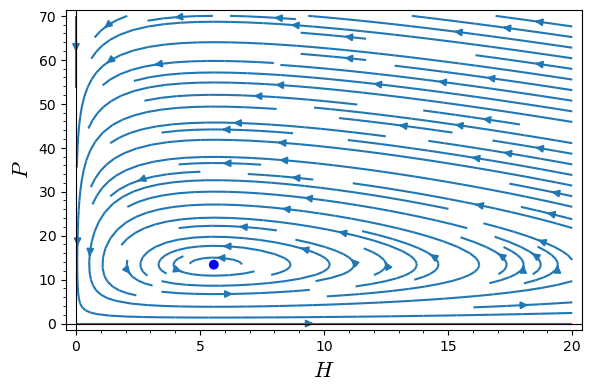
\includegraphics{Img/Plot example.png}
            \caption{Dinâmica do equilíbrio}
        \end{figure}
        
\newpage

\section{Pontos de equilíbrio}

Para encontrar os ponttos de equilíbrio das equações vamos resolver as EDOs. Fazendo a matriz das derivadas em relação à H e P chegamos:
$$\begin{bmatrix}
	r -pP & -pH\\
	apP & apH-d
	\end{bmatrix}$$
	
	e podemos encontrar os pontos onde as equações são iguais a 0. Isso acontece no ponto (0,0), como esperado, mas neste ponto sem população não é possível avanço do sistema. Outro ponto em que isso acontece é $(\frac{d}{ap}, \frac{r}{p})$. Substituindo esses valores na matriz, encontramos:
	$$\begin{bmatrix}
	0 & -\frac{d}{a}\\
	ra & 0
	\end{bmatrix}$$
	que, como o traço é 0 e o determinante positivo, é um ciclo. Podemos checar esse comportamento nos plots a seguir.
	
	O gráfico à esquerda representa a dinâmica do equilíbrio, onde o eixo horizontal representa a quantidade de Hospedeiros e o eixo vertical a quantidade de Parasitas. O gráfico a direita a curva em azul representa a quantidade de Hospedeiros e a curva em vermelho a quantidade de parasitas ao longo do tempo.
	
	Nessa primeira dinâmica iniciamos com 20 hospedeiros e 20 parasitoides. O ponto de equilíbrio central (em azul) é (10,10).

	
\begin{figure}[h!]
\begin{center}
	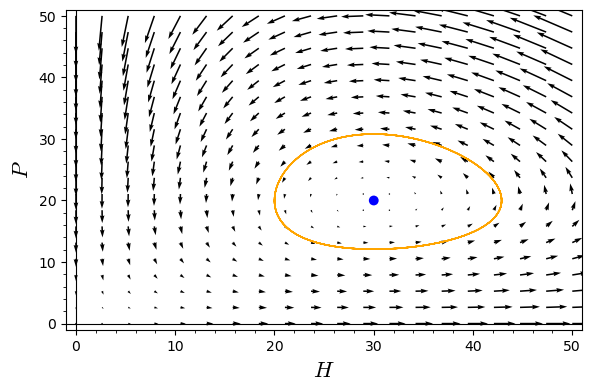
\includegraphics[height=5.4cm]{Img/HP (r=1,p=0.05, d=1.5,a=1); (20, 20); (30, 20).png} \quad
	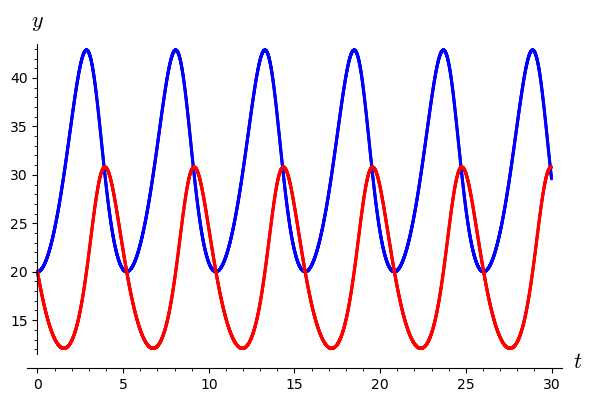
\includegraphics[height=5.4cm]{Img/T (r=1,p=0.05, d=1.5,a=1); (20, 20); (30, 20).png}
\caption{Plot r=1, p=0.05, d=1.5, a=1} \label{gdimotes}
\end{center}
\end{figure}


\newpage

Na segunda dinâmica iniciamos com 5 hospedeiros e 40 parasitoides. O ponto de equilíbrio central (em azul) é (10,10). Podemos observar que mesmo com menor eficiência de ingestão do parasita, pela pequena quantidade inicial de Hospediros, a quantidade de hospedeiros e parasitoides quase se extingue, mas isso não acontece.
\begin{figure}[h!]
\begin{center}
	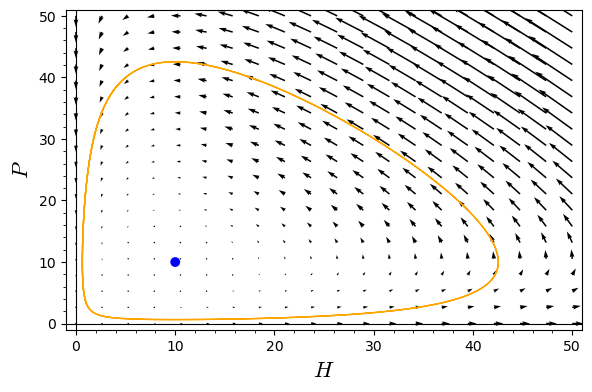
\includegraphics[height=5.4cm]{Img/HP (r=1,p=0.1, d=1,a=1); (5, 40); (10, 10).png} \quad
	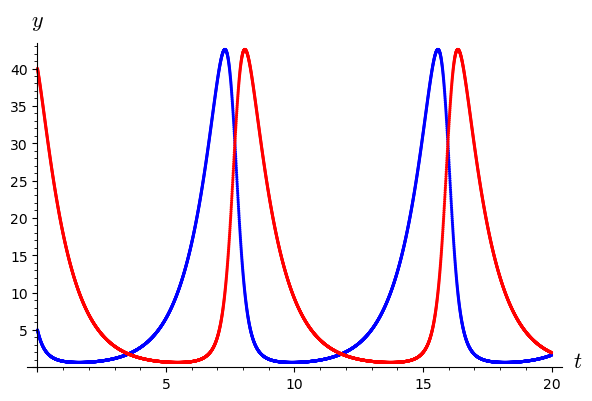
\includegraphics[height=5.4cm]{Img/T (r=1,p=0.1, d=1,a=1); (5, 40); (10, 10).png}
\caption{Plot r=1, p=0.1, d=1, a=1} \label{gdimotes}
\end{center}
\end{figure}


A seguir temos mais alguns plots. Na terceira dinâmica iniciamos com 30 hospedeiros e 80 parasitoides. O ponto de equilíbrio central é (100,80). Na quarta dinâmica iniciamos com 150 hospedeiros e 80 parasitoides. O ponto de equilíbrio central é (200,80). Na quinta dinâmica iniciamos com 300 hospedeiros e 80 parasitoides. O ponto de equilíbrio central é (400,120).

Podemos observar que as quantidades de hospedeiros e parasitoides nunca vão ser fixas, ou seja, não vai convergir, a não ser que o ponto inicial seja exatamente o ponto de equilíbrio, caso contrário o equilíbrio será um ciclo. Com essas equações, independente dos valores dos parâmetros, não temos pontos de bifurcação.
\newpage

\begin{figure}[h!]
\begin{center}
	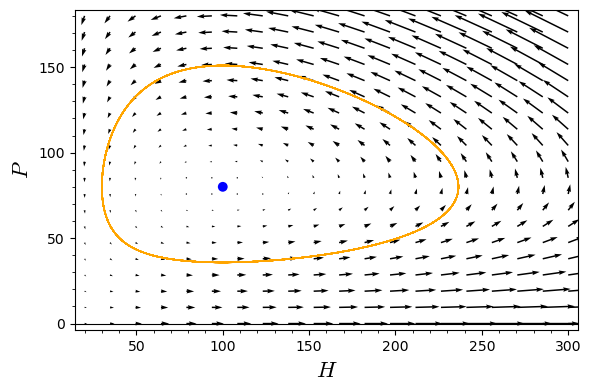
\includegraphics[height=5.4cm]{Img/HP (r=1.6,p=0.02, d=0.8,a=0.4); (30, 80); (100, 80).png} \quad
	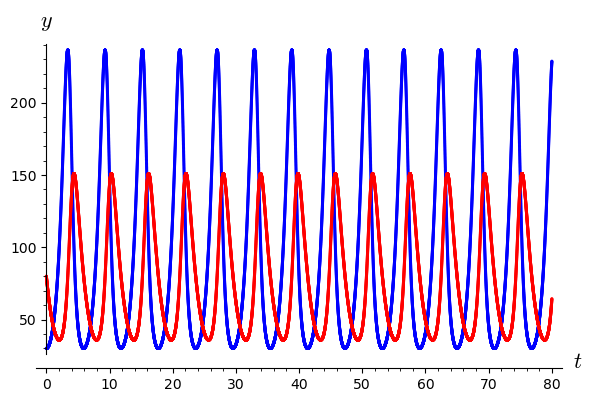
\includegraphics[height=5.4cm]{Img/T (r=1.6,p=0.02, d=0.8,a=0.4); (30, 80); (100, 80).png}
\caption{Plot r=1.6, p=0.02, d=0.8, a=0.4} \label{gdimotes}
\end{center}
\end{figure}



\begin{figure}[h!]
\begin{center}
	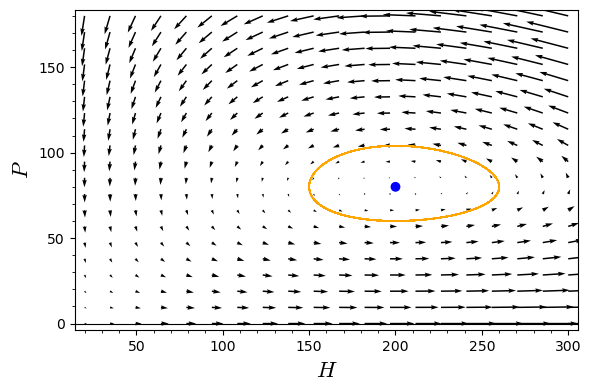
\includegraphics[height=5.4cm]{Img/HP (r=1.6,p=0.02, d=1.6,a=0.4); (150, 80); (200, 80).png} \quad
	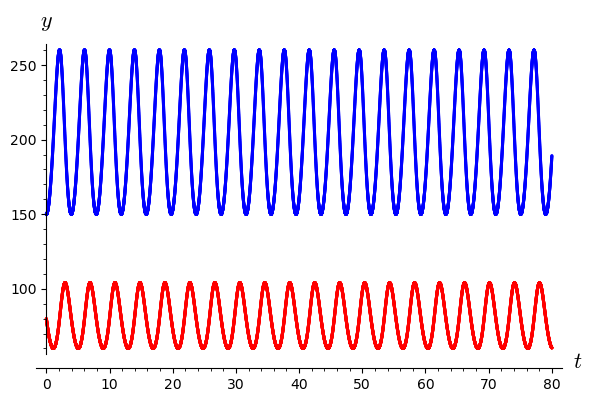
\includegraphics[height=5.4cm]{Img/T (r=1.6,p=0.02, d=1.6,a=0.4); (150, 80); (200, 80).png}
\caption{Plot r=1.6, p=0.02, d=1.6, a=0.4} \label{gdimotes}
\end{center}
\end{figure}

\begin{figure}[h!]
\begin{center}
	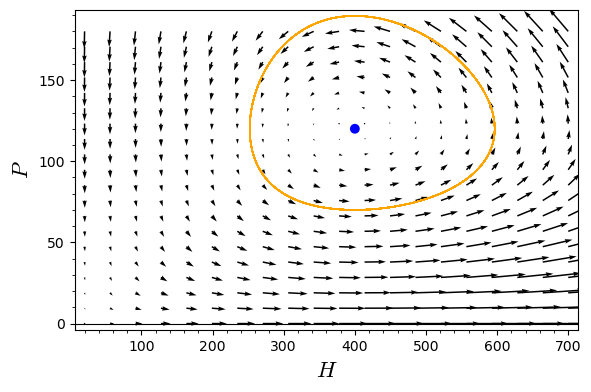
\includegraphics[height=5.4cm]{Img/HP (r=1.2,p=0.01, d=1.6,a=0.4); (300, 80); (400, 120).png} \quad
	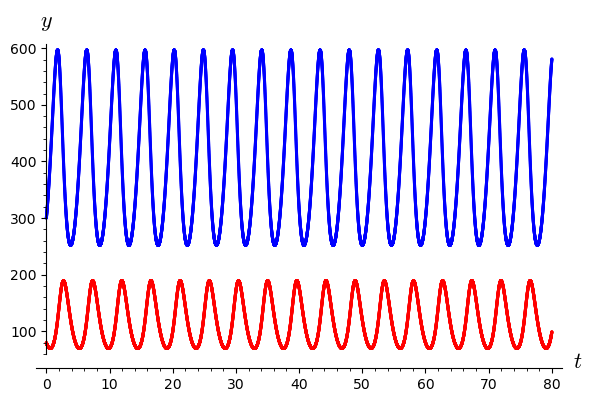
\includegraphics[height=5.4cm]{Img/T (r=1.2,p=0.01, d=1.6,a=0.4); (300, 80); (400, 120).png}
\caption{Plot r=1.2, p=0.01, d=1.6, a=0.4} \label{gdimotes}
\end{center}
\end{figure}

\newpage
        
\section{Discussão}
Temos então um campo de vetores no formato de um ciclo para cada uma das 5 simulações feitas, tendo elas seu próprio equilíbrio e valor inicial, mostrando como as populações se comportam a partir deste mesmo valor. Na Figura 2, apesar de seu valor inicial começar igual para ambas as populações, é visível que a população de hospedeiros se sobressai em relação aos parasitoides em quase todo o momento, isso provavelmente se deve pelo fato que a taxa de mortalidade $d$ que é a maior taxa em relação às outras. Na figura 2 temos que ao mudar os valores de $p$ para $0.1$ e $d$ para $1$, o ponto de equilíbrio se desloca em direção a origem e a variação de ambas populações fica muito maior quanto mais distante da mesma, o ponto inicial escolhido foi um teste para ver a possibilidade de extinção das espécies, algo que não parece possível neste modelo, já que com 8 vezes mais parasitoides do que hospedeiros não causou a extinção do segundo e logo após a extinção do primeiro, que apesar de se aproximarem de 0, não acabam por chegar em tal valor.

Pegando valores completamente novos, é visto que na Figura 4 um equilíbrio para valores um pouco maiores de hospedeiros e parasitoides comparado com os anteriores, apresentando a mesma característica dos gráficos da Figura 1, onde os valores de hospeiros em sua maioria ficam acima dos valores de parasitoides, além disso é perceptível que ambos valores de hospeiros e parasitoides no ponto de equilíbrio são valores inversamente proporcionais ao valor da eficiência de ingestão $p$ do parasitoide. A Figura 5 tem apenas o parâmetro $d$ de diferente com o gráfico anterior,  sendo que o parâmetro da Figura 5 tem o dobro de taxa de mortalidade do parasitoide, o que ironicamente não muda exatamente nada no ponto de equilíbrio do parasitoide, porém aumenta o equilíbrio do hospedeiro, sendo interpretado como uma prosperidade na população desses em relação a uma maior mortalidade de seus predadores, detalhe que no ponto inicial escolhido o número de hospedeiros sempre será maior que o número de predadores. Para finalizar vemos que ao diminuir a eficiência de ingestão $p$ junto com a natalidade de hospedeiros $r$ gerou um ponto de equilíbrio muito maior para ambas as populações, como mostrado na Figura 6, algo trivial  de se entender para população de hospedeiros, já  pra a populações de parasitoides, seguindo a lógica, além de ter mais hospedeiros para os parasitoides se reproduzirem/alimentar os danos causados por seus ataques são menores, causando uma prosperidade maior em sua população.

Uma característica destas simulações  é a impossibilidade de extinção entre os Hospedeiros e Parasitoides, tendo em vista que uma diminuição de H terá como consequência a diminuição da resposta funcional, já que a mesma é uma função de crescente a partir de H e P, causando então uma diminuição de P pelo fato da resposta funcional estar sendo adicionada a sua derivação, porém essa diminuição causará um aumento em H, pois a resposta funcional subtrai a derivada de H. O aumento de H por sua vez traz o aumento da resposta funcional,  aumentando P e impedindo que seu valor chegue a 0, assim aumentando a resposta funcional, o que por sua vez diminui H e assim segue o ciclo.  Isso facilmente é  interpretável no mundo real, onde o aumento de parasitas diminui o número de hospedeiros, o que cria uma escassez de alimentos para os parasitas, causando assim uma diminuição em seu número, isso enquanto os hospedeiros prosperam em têm um aumento em sua população pela diminuição de seu predador natural, o que por consequência acaba com a escassez de alimentos para os parasitas, fazendo os mesmos aumentarem em número. Essa interação é  muito necessário  para a análise do controle biológico, feito a partir do uso de parasitoides, já que necessariamente aumentar o número de parasitoides a partir de meios externos, em uma população fará com que em determinado período de tempo o número de hospedeiros seja bem muito reduzido, tendo em vista a mudança da interação feita entre os seres vivos, onde no modelo temos interpretado como a resposta funcional, um exemplo seria uma tentativa de diminuir a população de mosquitos (Hospedeiro) a partir da população de ácaros (Parasitoides).


\section{Conclusão}

Podemos ver que o modelo, sem intervenções externas, a partir de uma quatidade inicial positiva de hospedeiros e parasitoides vai ser um equilíbrio em ciclos periódicos, onde não existe extinção ou explosão na quantidade de um ou de ambos indivíduos. Assim, como exemplo, em uma região, quando os níveis de parasitoides estiverem acima de uma quantidade considerada maléfica, pode ocorrer uma intervenção para que haja o controle de parasitoides. Mas como é de conhecimento geral o sistema raramente é um ciclo, principalmente em populações de hospedeiros e parasitoides.

As análises feitas estão limitadas pela falta de dados concretos sobre as quantidades de indivíduos nas popupações reais, algo que é muito difícil de ser medido mesmo em um ambiente controlado. Se for considerada a possibilidade de interveção externa (que pode ocorrer de diversas formas), podem ocorrer casos onde uma ou ambas as expécies entrem em extinção. Além disso, nas análises apresentadas existem apenas uma expécie de hospedeiro e outra de parasitoide, algo que pode variar muito de acordo com o ambiente. Além disso, com o passar do tempo o hospedeiro pode se tornar mais resistente ao parasitoide pela seleção natural ou o parasita pode se tornar mais eficaz no ataque ao hospedeiro pelo mesmo motivo, no modelo é dado que esse valor é contante, a cada sistema, ao longo de todo o ciclo.

Existem diversas maneiras de se controlar um parasitoide, desde a liberação de predadores naturais até a utilização de produtos químicos, mas para que essa intervenção seja “adicionada” às equações das populações é necessária a observação de casos inde essas intervenções são feitas e estudar suas consequências. Com isso seria possível chegar ao melhor monento para tais intervenções e qual tipo de intervenção vai ser menos prejudicial e mais eficaz. Para análises com mais de um tipo de hospedeiro e parasitoide é necessário que haja o estudo de como os indivíduos interagem entre si, algo que se torna exponencialmente mais difícil a cada nova espécie adicionada ao sistema pois vai poder se relacionar com cada uma das já existentes no modelo. Para observar a diferença de eficácia do hospedeiro ou parasitoide no modelo são necessárias mais observações de como esses indivíduos se modificam ao longo do tempo.

Com isso é possível concluir que ainda é necessário muito estudo no modelo Hospedeiro-parasitoide, pois o mundo está em mudança e a ciência deve se manter atualizada e de acordo com os fatores que estão sendo estudados.


\section{Referências}

(1) LIMA, Ernesto; FERREIRA, Cláudia; GODOY, Wesley. Ecological Modeling and Pest Population Management: a Possible and 
Necessary Connection in a Changing World. Neotropical Entomology, Botucatu, v. 38, n. 6, p. 699 - 707, nov/dec. 2009.

\medskip

(2) Alharbi, W., Sandhu, S.K., Areshi, M. et al. Ecological Modeling and Pest Population Management. Sci Rep 12, 15023 (2022). https://doi.org 10.1038/s41598-022-18120-z

\medskip

(3) HOVESTADT Thomas. Multiple host use and the dynamics of host switching in host–parasite systems. Insect Conservation and Diversity, Wallingford, v. 12, p. 511 - 522, 2019.

\medskip

(4) Mills, N.J., Getz, W.M. Modelling the biological control of insect pests: a review of host-parasitoid models. Mathematical Biology Group. 2018. Disponível em: https://www.colorado.edu/project/mathbio/2018/
05/02/host-parasitoid-models. Acesso em: 12 de set. de 2022. 

\medskip

(5) STEVENS Hank. Primer of Ecology using R. 2022. Disponível em: https://hankstevens.github.io/Pri
mer-of-Ecology/host-parasitoid-relations.html. Acesso em: 12 de set. de 2022.

\medskip

(6) GORDON Harold. Slideshare: O modelo de Lotka e Volterra da predação.Disponível em: https:// pt.slideshare.net/popecologia/lotka-volterra-predao